\chapter{实验结果与分析}

\section{实验参数与负载配置}

本章实验使用 Locust~2.43.4 对三条链路各执行四象限压测，每次持续 600\,s，三链路顺序执行，时间覆盖 2026-05-12 00:31 至 02:52。负载分为低压与高压两档：低压统一设定为 3 并发用户、spawn rate 1\,user/s；高压根据链路特性调整，链路~A 约 5 并发，链路~B 因采用 AG-UI SSE 长连接协议吞吐敏感性更高，实际达到约 1.8\,req/s（10 并发），链路~C 约 5 并发。

本次实验的所有服务、负载脚本与可观测组件均运行在同一台 Ubuntu~22.04.5~LTS 主机上，内核版本为 Linux~5.15.0-131-generic。主机 CPU 为 Intel(R) Xeon(R) Platinum，分配 8 个逻辑核心，内存约 29\,GiB；显卡为 Cirrus Logic GD~5446 虚拟显示设备，实验过程未使用独立 GPU 加速。Python 服务与 Locust 脚本通过 \code{uv} 管理运行环境，项目声明并使用 CPython~3.12 系列环境，主要依赖包括 Locust、FastAPI、LangGraph、Google ADK、gRPC、OpenTelemetry、Pandas 与 PyYAML 等。前端与网关相关 TypeScript 组件运行在 Node.js~20.18.2 环境下，主要依赖包括 Next.js、React、AG-UI、CopilotKit、\code{@grpc/grpc-js} 与 OpenTelemetry 相关库。

表~\ref{tab:experiment-env} 给出本章实验环境。实验目标不是测量 TripSphere 的容量上限，而是在可控负载下比较 baseline 与 fault 条件的系统响应差异，因此本文更关注同一链路内部的相对变化、故障命中证据和业务质量指标。

\begin{table}[htbp]
  \centering
  \small
  \caption{实验环境与主要依赖}
  \label{tab:experiment-env}
  \begin{tabularx}{\textwidth}{p{3.2cm}X}
    \toprule
    项目 & 配置 \\
    \midrule
    操作系统 & Ubuntu 22.04.5 LTS（Linux 5.15.0-131-generic） \\
    硬件环境 & Intel(R) Xeon(R) Platinum，8 逻辑核心，约 29\,GiB 内存，无独立 GPU 加速 \\
    负载工具 & Locust 2.43.4 \\
    Java 服务 & OpenJDK 11.0.30，Maven Wrapper 管理的 Spring Boot gRPC 微服务 \\
    Python 服务 & \code{uv} 管理的 CPython 3.12 系列 LangGraph/ADK Agent 服务 \\
    TypeScript 服务 & Node.js 20.18.2，前端与网关相关组件 \\
    可观测组件 & OpenTelemetry SDK、Tempo Trace 查询、实验质量 CSV \\
    实验控制 & \code{x-experiment-id}、\code{x-fault-scenario} 与故障配置文件 \\
    \bottomrule
  \end{tabularx}
\end{table}

各链路的故障场景如下。链路~A 使用组合故障 \code{chaina\_final}：地理编码延迟 5\,s（概率 0.5）、景点 RPC 异常（概率 0.4）、行程持久化返回 \code{UNAVAILABLE}（概率 0.2）。链路~B 使用组合故障 \code{chainb\_final}：chat agent LLM 异常（概率 0.4）、\code{itinerary} 状态清空（概率 0.25）、\code{pending\_day\_plan} 状态清空（概率 0.35）。链路~C 使用组合故障 \code{chainc\_final}：A2A Trace 断链（概率 0.3）、order assistant LLM 异常（概率 0.4）、商品 RPC 错误（概率 0.3）、订单草稿清空（概率 0.2）。

业务质量数据来源于实验随路记录的质量 CSV，降级判定与信号抽取由降级报告脚本完成；HTTP 性能指标来源于 Locust 生成的统计 CSV。本文采用的核心指标包括：HTTP 失败率、端到端 p50/p95 延迟、无降级率、降级率、链路~B 的 StateSnapshot 更新率以及链路~C 的订单提交率。其中，HTTP 失败率衡量传输层和入口层是否返回错误；降级率衡量请求是否出现内容缺失、状态未更新、fallback 或业务副作用缺失；StateSnapshot 更新率衡量前端能否收到有效状态同步；订单提交率衡量跨 Agent 链路是否完成最终业务副作用。这些指标共同构成“HTTP 指标 + 业务质量指标”的实验评价框架。

\section{三链路实验结果}

表~\ref{tab:overview} 汇总三条链路全部 12 次实验的关键指标。链路~B 和链路~C 在所有条件下 HTTP 失败率均为 0\%，但业务质量指标与 baseline 之间存在显著差异。两条链路的故障完全绕过了 HTTP 层，对传统基于响应码的监控不可见。

\begin{table}[htbp]
  \centering
  \scriptsize
  \caption{三链路四象限实验总览}
  \label{tab:overview}
  \resizebox{\textwidth}{!}{%
  \begin{tabular}{llrrrrrrl}
    \toprule
    链路 & 象限 & 请求数 & 失败数（率） & p50\,(ms) & p95\,(ms) & 无降级率 & 降级率 & 业务关键指标 \\
    \midrule
    A & baseline-low  &  76 &  1\,(1.3\%)   & 34\,000 & 57\,000 & 88.2\% & 10.5\% & 无持久化失败 \\
    A & baseline-high & 288 &  8\,(2.8\%)   & 37\,000 & 56\,000 & 89.6\% &  7.6\% & 无持久化失败 \\
    A & fault-low     &  68 & 25\,(36.8\%)  & 38\,000 & 60\,000 & 32.4\% & 30.9\% & geocoding\_fallback 主导 \\
    A & fault-high    & 272 & 108\,(39.7\%) & 40\,000 & 59\,000 & 29.7\% & 30.4\% & geocoding\_fallback 主导 \\
    \midrule
    B & baseline-low  &   139 & 0\,(0\%) &  3\,300 & 30\,000 & 97.1\% &  2.9\% & StateSnapshot 更新率 97.8\% \\
    B & baseline-high &   451 & 0\,(0\%) &  3\,700 & 30\,000 & 96.0\% &  4.0\% & StateSnapshot 更新率 97.3\% \\
    B & fault-low     &   341 & 0\,(0\%) &  1\,500 &  5\,000 & 39.3\% & 60.7\% & StateSnapshot 更新率 56.9\% \\
    B & fault-high    & 1\,077 & 0\,(0\%) & 1\,600 &  6\,200 & 44.2\% & 55.8\% & StateSnapshot 更新率 62.6\% \\
    \midrule
    C & baseline-low  &  84 & 0\,(0\%) & 14\,000 & 29\,000 & 98.8\% &  1.2\% & 订单提交率 98.8\% \\
    C & baseline-high & 131 & 0\,(0\%) & 15\,000 & 29\,000 & 96.4\% &  3.6\% & 订单提交率 96.4\% \\
    C & fault-low     & 129 & 0\,(0\%) &  5\,100 & 16\,000 &  3.8\% & 96.2\% & 订单提交率\,\textbf{3.8\%} \\
    C & fault-high    & 208 & 0\,(0\%) & 11\,000 & 27\,000 &  5.6\% & 94.4\% & 订单提交率\,\textbf{5.6\%} \\
    \bottomrule
  \end{tabular}}
\end{table}

\begin{figure}[htbp]
  \centering
  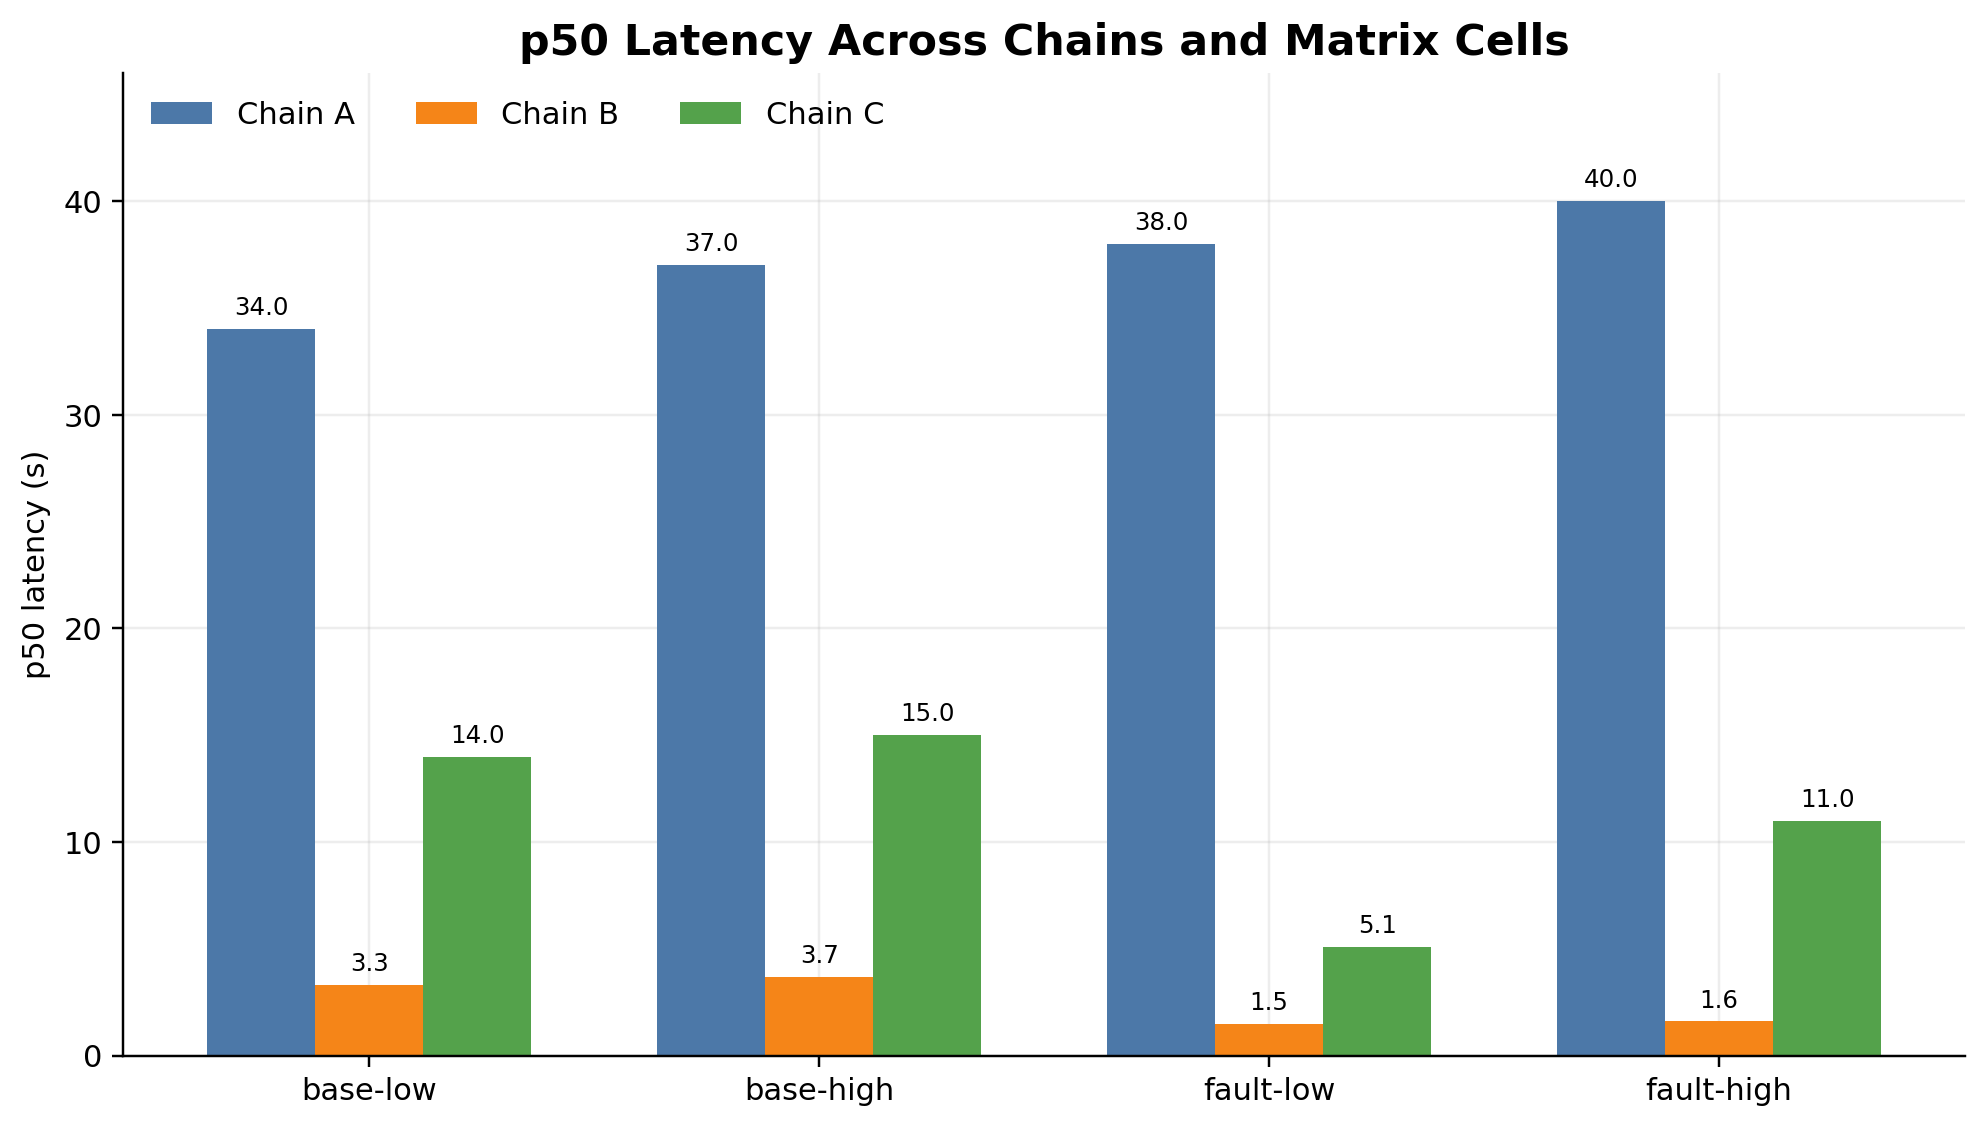
\includegraphics[width=\textwidth]{figures/exp-p50-latency-compare.png}
  \caption{三链路四象限 p50 延迟对比}
  \label{fig:p50-compare}
\end{figure}

\begin{figure}[htbp]
  \centering
  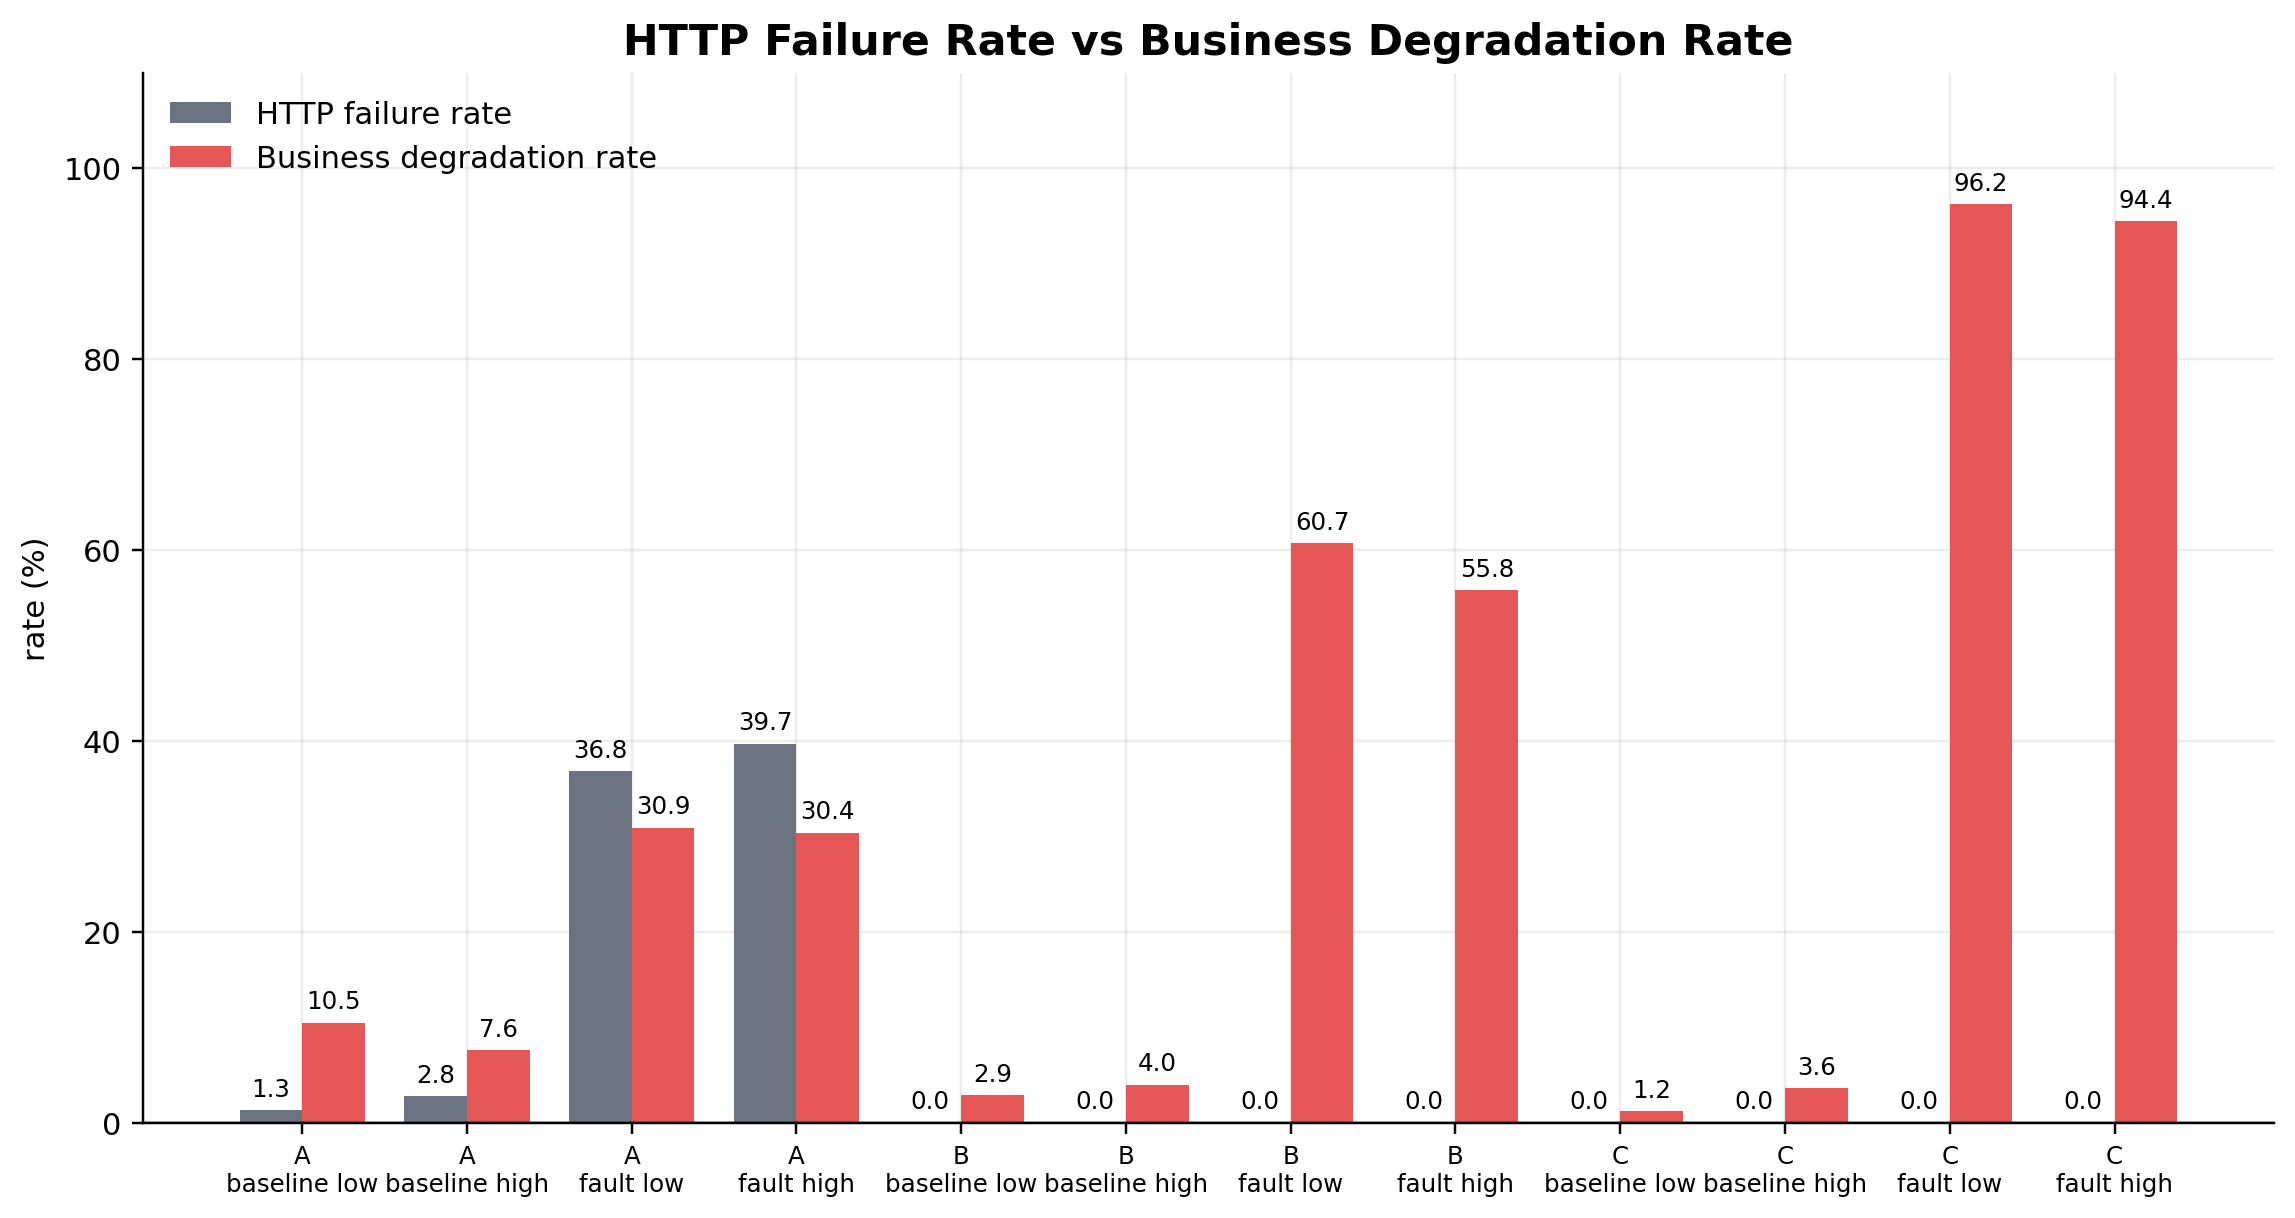
\includegraphics[width=\textwidth]{figures/exp-http-failure-vs-degradation.png}
  \caption{HTTP 失败率与业务降级率对比}
  \label{fig:http-vs-degradation}
\end{figure}

\noindent\textbf{链路 A 详细数据。}
表~\ref{tab:chaina-latency} 给出链路~A 各象限的完整延迟百分位与失败吞吐。故障组 p99 显著跳升至 79\,000--130\,000\,ms，来自 gRPC \code{UNAVAILABLE} 错误在持久化阶段的超时等待。

\begin{table}[htbp]
  \centering
  \footnotesize
  \caption{链路 A 延迟百分位详表（单位：ms，fail/s 为 Locust 失败吞吐）}
  \label{tab:chaina-latency}
  \begin{tabularx}{\textwidth}{p{2.4cm}XXXXXXXX}
    \toprule
    象限 & p50 & p75 & p90 & p95 & p98 & p99 & avg & fail/s \\
    \midrule
    baseline-low  & 35\,000 & 42\,000 & 49\,000 & 57\,000 &  75\,000 & 124\,000 & 35\,965 & 0.002 \\
    baseline-high & 37\,000 & 45\,000 & 51\,000 & 56\,000 &  68\,000 &  85\,000 & 37\,865 & 0.013 \\
    fault-low     & 38\,000 & 44\,000 & 53\,000 & 60\,000 &  98\,000 & 130\,000 & 39\,646 & 0.042 \\
    fault-high    & 40\,000 & 47\,000 & 54\,000 & 59\,000 &  66\,000 &  79\,000 & 40\,053 & 0.182 \\
    \bottomrule
  \end{tabularx}
\end{table}

表~\ref{tab:chaina-quality} 给出按降级状态分组的延迟与内容质量指标。baseline 组降级请求（sparse activities）的 p50 约为 12\,000--13\,000\,ms，远低于正常请求，系 AI Provider 内容审查在生成阶段提前返回所致，属背景噪声，不计入注入效果分析。fault 组降级请求的 p50 与无降级请求相近，说明 geocoding 延迟注入后仍需运行完整 LLM 推理流程。

\begin{table}[htbp]
  \centering
  \scriptsize
  \caption{链路 A 业务质量分组指标}
  \label{tab:chaina-quality}
  \resizebox{\textwidth}{!}{%
  \begin{tabular}{lrrrrrrrrr}
    \toprule
    象限 & p50-全 & p95-全 & p50-正常 & p95-正常 & p50-降级 & p95-降级 & 天数 & 活动 & Markdown \\
    \midrule
    baseline-low  & 34\,465 & 57\,109 & 36\,657 & 57\,109 & 12\,833 & 16\,487 & 3.0 & 11.0 & 1\,764 \\
    baseline-high & 37\,103 & 56\,337 & 38\,295 & 56\,785 & 11\,833 & 18\,249 & 3.0 & 11.3 & 1\,791 \\
    fault-low     & 37\,610 & 60\,433 & 38\,031 & 62\,345 & 37\,310 & 54\,899 & 3.0 & 11.4 & 1\,779 \\
    fault-high    & 39\,903 & 59\,433 & 42\,258 & 64\,646 & 36\,507 & 55\,706 & 3.0 & 11.7 & 1\,804 \\
    \bottomrule
  \end{tabular}}
\end{table}

\begin{table}[htbp]
  \centering
  \small
  \caption{链路 A 降级信号分布}
  \label{tab:chaina-signals}
  \begin{tabularx}{\textwidth}{p{2.5cm}p{1.8cm}p{4cm}X}
    \toprule
    象限 & 降级总数 & geocoding\_fallback（数/占比） & sparse\_activities（数/占比） \\
    \midrule
    baseline-low  &  8 &  0\,/\,0\%    &  8\,/\,100\% \\
    baseline-high & 22 &  0\,/\,0\%    & 22\,/\,100\% \\
    fault-low     & 21 & 18\,/\,85.7\% &  3\,/\,14.3\% \\
    fault-high    & 83 & 77\,/\,92.8\% &  6\,/\,7.2\% \\
    \bottomrule
  \end{tabularx}
\end{table}

\noindent\textbf{链路 B 详细数据。}
表~\ref{tab:chainb-latency} 给出链路~B 各象限延迟百分位。fault 组所有百分位均低于 baseline 组，p50 从 3\,300--3\,700\,ms 降至 1\,500--1\,600\,ms，p95 从 30\,000\,ms 降至 5\,000--6\,200\,ms。

\begin{table}[htbp]
  \centering
  \footnotesize
  \caption{链路 B 延迟百分位详表（单位：ms）}
  \label{tab:chainb-latency}
  \begin{tabularx}{\textwidth}{p{2.4cm}XXXXXXXX}
    \toprule
    象限 & p50 & p75 & p90 & p95 & p98 & p99 & avg & RPS \\
    \midrule
    baseline-low  & 3\,300 & 17\,000 & 24\,000 & 30\,000 & 40\,000 & 46\,000 &  9\,162 & 0.23 \\
    baseline-high & 3\,700 & 18\,000 & 24\,000 & 30\,000 & 37\,000 & 46\,000 &  9\,462 & 0.75 \\
    fault-low     & 1\,500 &  2\,700 &  4\,000 &  5\,000 &  6\,900 & 14\,000 &  1\,777 & 0.57 \\
    fault-high    & 1\,600 &  2\,800 &  3\,900 &  6\,200 & 11\,000 & 14\,000 &  2\,035 & 1.80 \\
    \bottomrule
  \end{tabularx}
\end{table}

表~\ref{tab:chainb-quality} 给出链路~B 分组质量指标。降级请求的 p50 在 baseline-low 时仅 8\,ms，在 fault-low 时为 105\,ms，证实了 fail-fast 快速返回路径的存在。全程 RUN\_ERROR 为 0，表明故障完全发生在应用语义层。

\begin{table}[htbp]
  \centering
  \scriptsize
  \caption{链路 B 业务质量分组指标}
  \label{tab:chainb-quality}
  \resizebox{\textwidth}{!}{%
  \begin{tabular}{lrrrrrrrrr}
    \toprule
    象限 & p50-全 & p95-全 & p50-正常 & p95-正常 & p50-降级 & p95-降级 & 均文本 & 均工具 & Snap 率 \\
    \midrule
    baseline-low  & 3\,296 & 29\,731 & 3\,306 & 29\,731 &     8 &  9\,221 & 102.9 & 2.7 & 97.8\% \\
    baseline-high & 3\,685 & 30\,034 & 3\,720 & 30\,104 &   749 & 22\,666 &  94.7 & 2.8 & 97.3\% \\
    fault-low     & 1\,463 &  4\,971 & 2\,734 &  6\,379 &   105 &  3\,233 &  23.9 & 0.5 & 56.9\% \\
    fault-high    & 1\,588 &  6\,162 & 2\,613 & 10\,588 &   198 &  4\,278 &  27.0 & 0.7 & 62.6\% \\
    \bottomrule
  \end{tabular}}
\end{table}

\begin{table}[htbp]
  \centering
  \small
  \caption{链路 B 降级信号分布（一个请求可触发多个信号）}
  \label{tab:chainb-signals}
  \begin{tabularx}{\textwidth}{p{2.4cm}p{1.8cm}p{3.2cm}p{3.2cm}X}
    \toprule
    象限 & 降级总数 & no\_response\_text & no\_state\_update & no\_tool\_calls \\
    \midrule
    baseline-low  &   4 &  4\,/\,100.0\% &   3\,/\,75.0\%  &   3\,/\,75.0\% \\
    baseline-high &  18 & 18\,/\,100.0\% &  12\,/\,66.7\%  &  12\,/\,66.7\% \\
    fault-low     & 207 & 205\,/\,99.0\% & 147\,/\,71.0\%  & 94\,/\,45.4\% \\
    fault-high    & 602 & 601\,/\,99.8\% & 404\,/\,67.1\%  & 269\,/\,44.7\% \\
    \bottomrule
  \end{tabularx}
\end{table}

\begin{figure}[htbp]
  \centering
  \includegraphics[width=\textwidth]{figures/exp-degradation-rate-compare.pdf}
  \caption{三链路四象限业务降级率对比}
  \label{fig:degradation-rate}
\end{figure}

\noindent\textbf{链路 C 详细数据。}
表~\ref{tab:chainc-latency} 给出链路~C 的延迟百分位。fault-low 的 p50 从约 15\,000\,ms 降至 5\,100\,ms，与链路~B 的延迟反转现象成因相同——LLM 异常快速失败路径主导整体分布。

\begin{table}[htbp]
  \centering
  \footnotesize
  \caption{链路 C 延迟百分位详表（单位：ms）}
  \label{tab:chainc-latency}
  \begin{tabularx}{\textwidth}{p{2.4cm}XXXXXXXX}
    \toprule
    象限 & p50 & p75 & p90 & p95 & p98 & p99 & avg & RPS \\
    \midrule
    baseline-low  & 15\,000 & 21\,000 & 24\,000 & 29\,000 & 32\,000 & 34\,000 & 16\,013 & 0.14 \\
    baseline-high & 15\,000 & 21\,000 & 26\,000 & 29\,000 & 36\,000 & 37\,000 & 16\,869 & 0.36 \\
    fault-low     &  5\,100 &  7\,600 & 14\,000 & 16\,000 & 18\,000 & 20\,000 &  6\,357 & 0.26 \\
    fault-high    & 11\,000 & 16\,000 & 23\,000 & 27\,000 & 33\,000 & 37\,000 & 12\,460 & 0.44 \\
    \bottomrule
  \end{tabularx}
\end{table}

\begin{table}[htbp]
  \centering
  \scriptsize
  \caption{链路 C 业务质量分组指标（†：单次挂起离群值，不具代表性）}
  \label{tab:chainc-quality}
  \resizebox{\textwidth}{!}{%
  \begin{tabular}{lrrrrrrrr}
    \toprule
    象限 & p50-全 & p95-全 & p50-正常 & p95-正常 & p50-降级 & p95-降级 & 草稿率 & 提交率 \\
    \midrule
    baseline-low  & 14\,467 &  28\,932   & 14\,242 &  28\,932   & 20\,151 & 20\,151 & 2.4\% & 98.8\% \\
    baseline-high & 15\,680 & 586\,256†  & 15\,684 & 586\,256†  & 12\,461 & 30\,961 & 2.9\% & 96.4\% \\
    fault-low     &  5\,143 &  16\,528   & 10\,414 &  23\,302   &  4\,898 & 16\,055 & 5.3\% &  3.8\% \\
    fault-high    & 11\,395 &  33\,432   & 14\,491 & 598\,720†  & 11\,165 & 27\,673 & 6.1\% &  5.6\% \\
    \bottomrule
  \end{tabular}}
\end{table}

\section{结果分析}

\noindent\textbf{链路 A：持久化无 Fallback 与 Geocoding 降级的传导。}
链路~A 的 baseline 组已存在约 7--11\% 的 \code{sparse\_activities} 降级率，该现象来自模型输出阶段的内容审查或网关波动，属于 AI 原生应用的环境背景噪声，与注入无关。在评估故障注入效果时需扣除此基线。故障注入后，HTTP 失败率从 baseline 的 1--3\% 跳升至 37--40\%，失败体均为 \code{\{"detail":"Failed to persist itinerary"\}}（HTTP~502）。这揭示出一个架构缺陷：链路~A 最终的 gRPC 持久化节点没有重试机制，一旦收到 \code{UNAVAILABLE} 错误即直接向上层返回 502，AI 内容生成阶段的所有工作全部浪费。

\code{geocoding\_fallback} 信号在降级请求中的占比（86--93\%）显著高于 geocoding 延迟注入的声明概率（50\%）。原因在于注入 5\,s 延迟后，几乎所有命中该注入点的请求都因超时而失去坐标数据，被迫转入关键词搜索的 fallback 路径。该 fallback 机制有效避免了硬失败，但会导致活动数从约 12 降至 3、Markdown 从 1\,800 字符降至 800 字符以内的内容质量退化。

\noindent\textbf{链路 B：延迟反转与状态静默污染。}
链路~B 的 HTTP 失败率在全部实验中恒为 0\%，HTTP 监控对该链路的所有退化完全失效。最具反常性的发现是“延迟反转”：故障条件下 p50 从 3\,300\,ms 降至 1\,500\,ms，p95 从 30\,000\,ms 降至 5\,000\,ms。根本原因在于：\code{llm.chat\_agent.exception} 以概率 0.4 注入时，LangGraph 节点在进入 LLM 调用前即抛出 RuntimeError 并立即终止，响应时间约 93--200\,ms。大量极速失败请求拉低了整体百分位分布，使系统在统计意义上“表现更快”，但实际上 60\% 以上的对话 turn 没有执行有效动作。

状态注入对前端 UI 的影响更为隐蔽：即使 LLM 调用正常响应，在 LangGraph reducer 归并状态时字段被清空，前端 StateSnapshot 收到 \code{null} 或空对象覆盖，用户看到行程页面清空，但系统日志和 HTTP 层均无任何错误信号。StateSnapshot 更新率从 97\% 降至 57--63\% 是捕获此类退化的关键指标。

\noindent\textbf{链路 C：串行故障叠加与可观测性断链。}
链路~C 的 HTTP 失败率与远端委托率在全部条件下分别保持在 0\% 和 100\%，从传统监控视角系统运行完美，而实际订单提交率从 baseline 的 98.8\% 暴跌至 fault-low 的 3.8\%，96.2\% 的请求业务失败。

这种数量级下降不能仅由各故障声明概率的独立相乘解释，而是来自提交链路中最上游 ReAct 步骤的短路放大：一旦 \code{order\_assistant} LLM 节点异常，后续商品查询、草稿创建与订单提交均不会发生。该现象的定量差距与 Trace 断链影响在案例二中进一步展开。

\noindent\textbf{跨链路对比。}
三条链路的 HTTP 层与业务层背离程度形成清晰梯度：链路~A 最“诚实”（HTTP~502 可感知持久化失败），链路~B 和链路~C 的 HTTP 层对所有退化完全透明，但链路~C 的业务崩溃程度（降级率 96\%）远超链路~B（60\%）。纯 HTTP 监控在链路~B/C 场景下完全失效，需要专门的业务质量探针：链路~A 需要 \code{itinerary\_saved\_rate} 和 \code{activity\_count}；链路~B 需要 \code{StateSnapshot} 更新率和 \code{tool\_calls\_count}；链路~C 需要 \code{order\_submit\_rate} 和 \code{order\_draft\_seen}。

\section{案例研究}

\subsection{案例一：链路 B——LLM 异常注入下的延迟反转与静默降级}

\textbf{实验背景}。本案例基于 chainb-fault-low（完整实验 ID 见 artifacts 目录中的同名运行记录），负载为低压 3 并发，600\,s，共 341 次 chat-turn 请求。故障 DSL 包含三个并发注入点：LLM 节点 RuntimeError（概率 0.4）、itinerary 状态清空（概率 0.25）、pending\_day\_plan 状态清空（概率 0.35）。

\textbf{现象}。p50 延迟从 baseline-low 的 3\,300\,ms 反向下降至 1\,500\,ms，p95 从 30\,000\,ms 降至 5\,000\,ms，HTTP 失败率维持 0\%。同时，业务质量急剧恶化：60.7\% 的 turn 发生降级，StateSnapshot 更新率从 97.8\% 骤降至 56.9\%，平均工具调用次数从 2.7 降至 0.5，平均响应文本从 102.9 字符降至 23.9 字符。

\textbf{数据证据}。\code{quality.csv} 请求时间线中存在两类典型降级模式：第一类是 elapsed $<$ 200\,ms 的极速失败，\code{text\_chars=0}，\code{tool\_calls=0}，\code{state\_snapshot\_seen=False}，对应 LLM exception 直接短路；第二类是 elapsed 约 1\,500--5\,000\,ms 的“工具完成但无输出”，\code{tool\_calls>=1}，\code{text\_chars=0}，对应异常发生在工具调用之后、结构化输出之前。

\textbf{根因分析}。LangGraph 节点内部捕获 RuntimeError 后立即终止该节点，返回空 \code{AIMessage}。AG-UI SSE 协议将流结束视为正常完成，无法区分有内容与无内容的流。\code{state.itinerary.clear} 和 \code{state.pending\_day\_plan.clear} 在 reducer 归并时将字段清零，前端 UI 无法区分“行程未加载”与“行程被静默清空”。整个退化过程在 HTTP 层和系统日志层均无可见信号。

\begin{figure}[htbp]
  \centering
  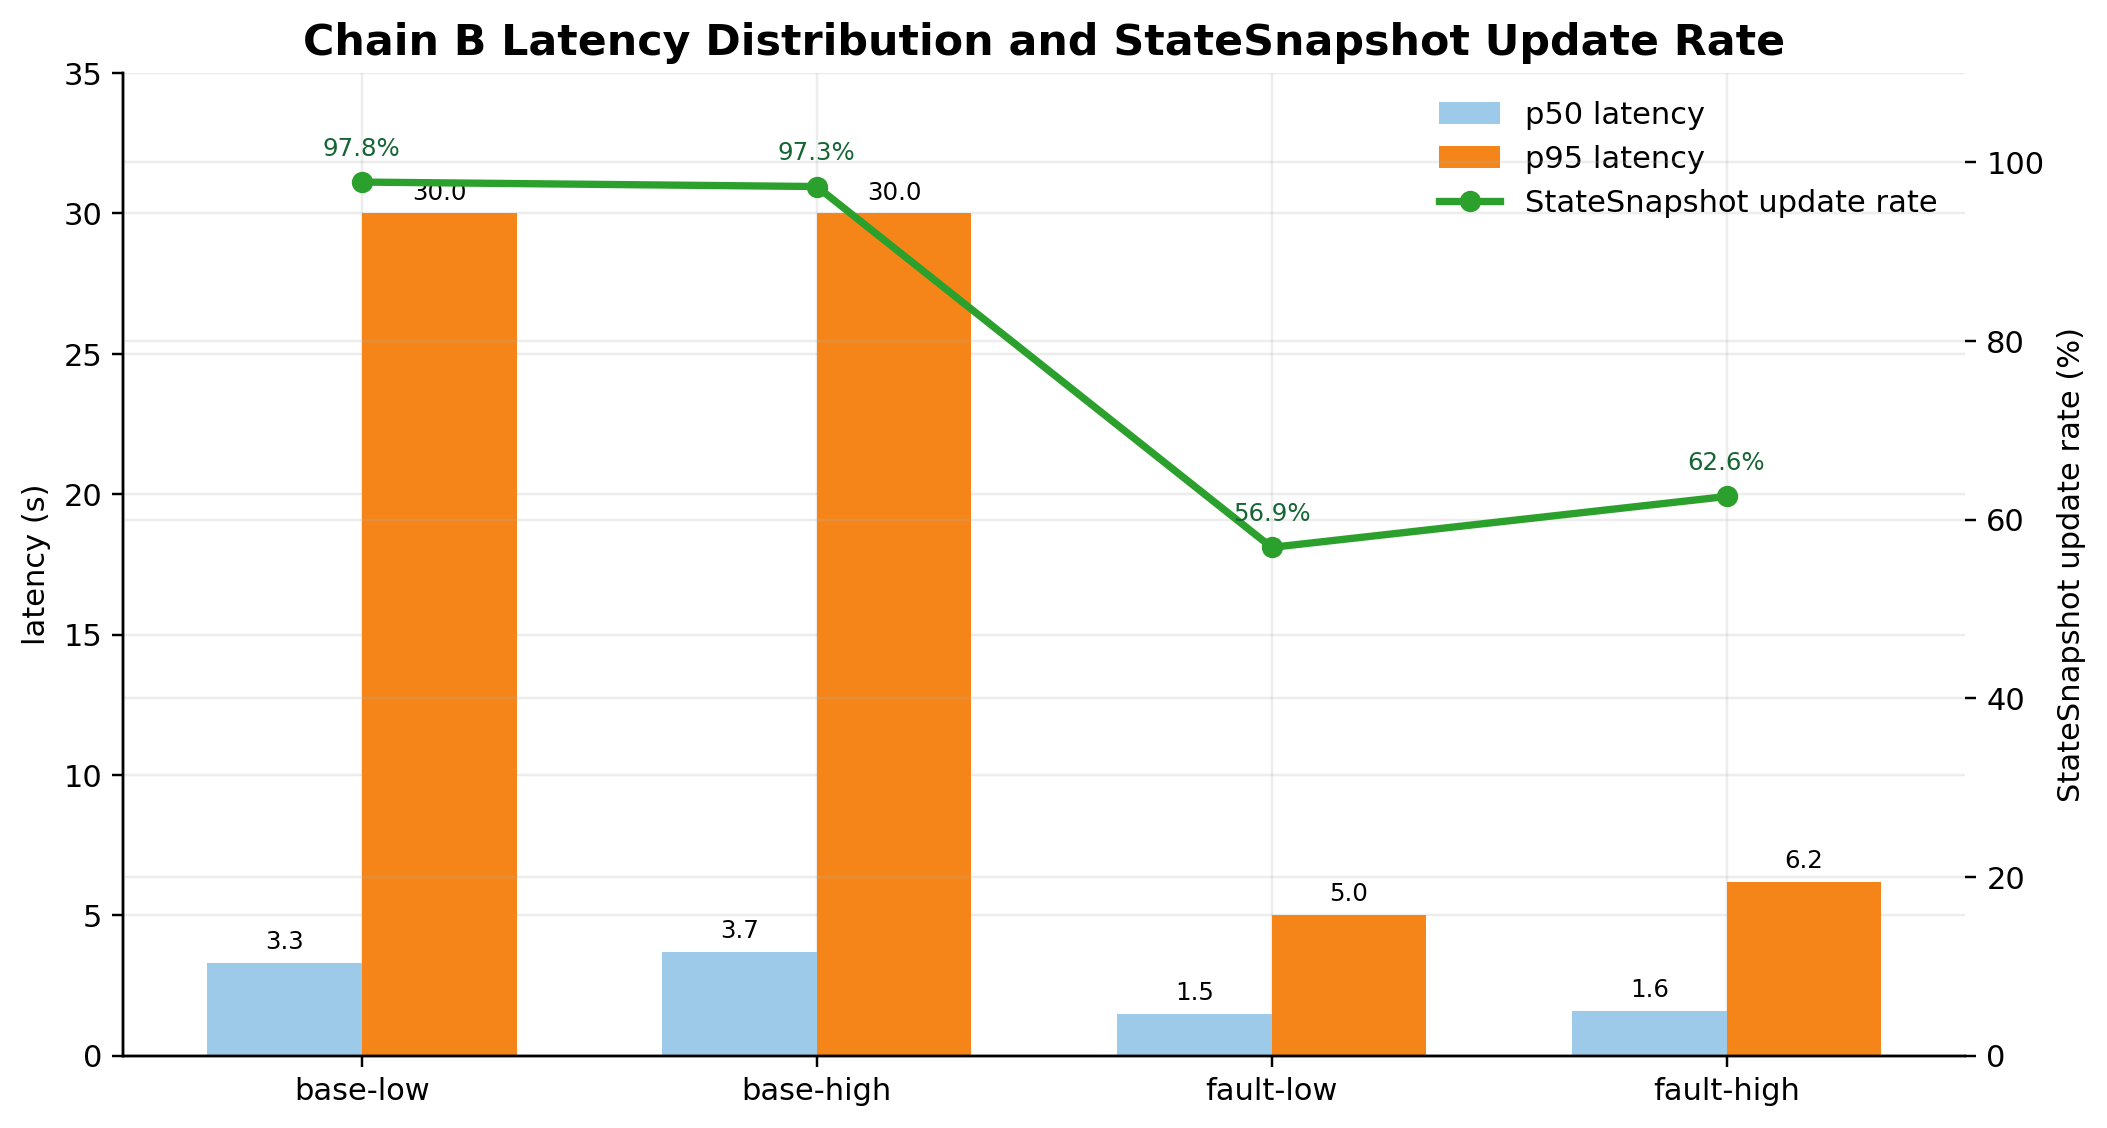
\includegraphics[width=\textwidth]{figures/case-chainb-latency-snapshot.png}
  \caption{链路 B 延迟分布与 StateSnapshot 更新率随象限变化}
  \label{fig:chainb-latency-snap}
\end{figure}

\subsection{案例二：链路 C——四点故障组合爆炸与订单流水线崩溃}

\textbf{实验背景}。本案例基于 chainc-fault-low（完整实验 ID 见 artifacts 目录中的同名运行记录），低压 3 并发，600\,s，共 131 次 order-submit 请求。同时激活四类故障：\code{order\_assistant} LLM RuntimeError（概率 0.4）、GetSkuById RPC \code{UNAVAILABLE}（概率 0.3）、\code{order\_draft} 状态清空（概率 0.2）、A2A Trace 断链（概率 0.3）。

\textbf{现象}。126/131 个请求的 \code{order\_submit} turn 以降级告终，订单提交率从 baseline-low 的 98.8\% 暴跌至 3.8\%。全程 HTTP 失败率 0\%，远端委托率 100\%——基础设施层监控无任何异常信号。

\textbf{理论与实测的差距}。若只考虑直接影响订单提交的三类业务故障，并假定每类故障在一次提交请求中独立命中一次，则成功率理论预期为：
\[
P_{\text{theory}} = (1-0.4)\times(1-0.3)\times(1-0.2) \approx 33.6\%
\]
但实测订单提交率仅 3.8\%，约为理论预期的 $\frac{1}{9}$。差距主要归因于 \code{order\_assistant} 的 LLM 节点并非“每个请求只判定一次”的普通故障点，而是 ReAct 提交流程的上游控制点：它负责决定是否调用 \code{GetSkuById}、是否形成订单草稿以及是否继续推进到 \code{CreateOrder}。因此，该节点一旦在任一关键推理步短路，请求不会进入后续商品查询和订单创建阶段，\code{GetSkuById} RPC 错误与 \code{state.order\_draft.clear} 的独立概率也失去原本的乘法意义。换言之，实测差距的核心不是四个故障概率简单叠加，而是 LLM 控制节点把一次异常放大为整条订单流水线的提前终止。

\textbf{预存 Bug 与可观测性断链}。即使不注入任何故障，\code{order\_assistant} 在 submit 阶段向 gRPC \code{CreateOrder} 发送的请求中 \code{items} 字段为空列表，服务端 validation 拒绝该请求（baseline-low 已有 1 次自然失败，占比 1.2\%）。同时，\code{a2a.trace.drop} 使部分失败请求的跨服务 Trace 关联被切断，在 Tempo 中仅可见 \code{trip-chat-service} 侧的根 Span，验证了可观测性本身的可靠性对故障归因的关键影响。

\begin{figure}[htbp]
  \centering
  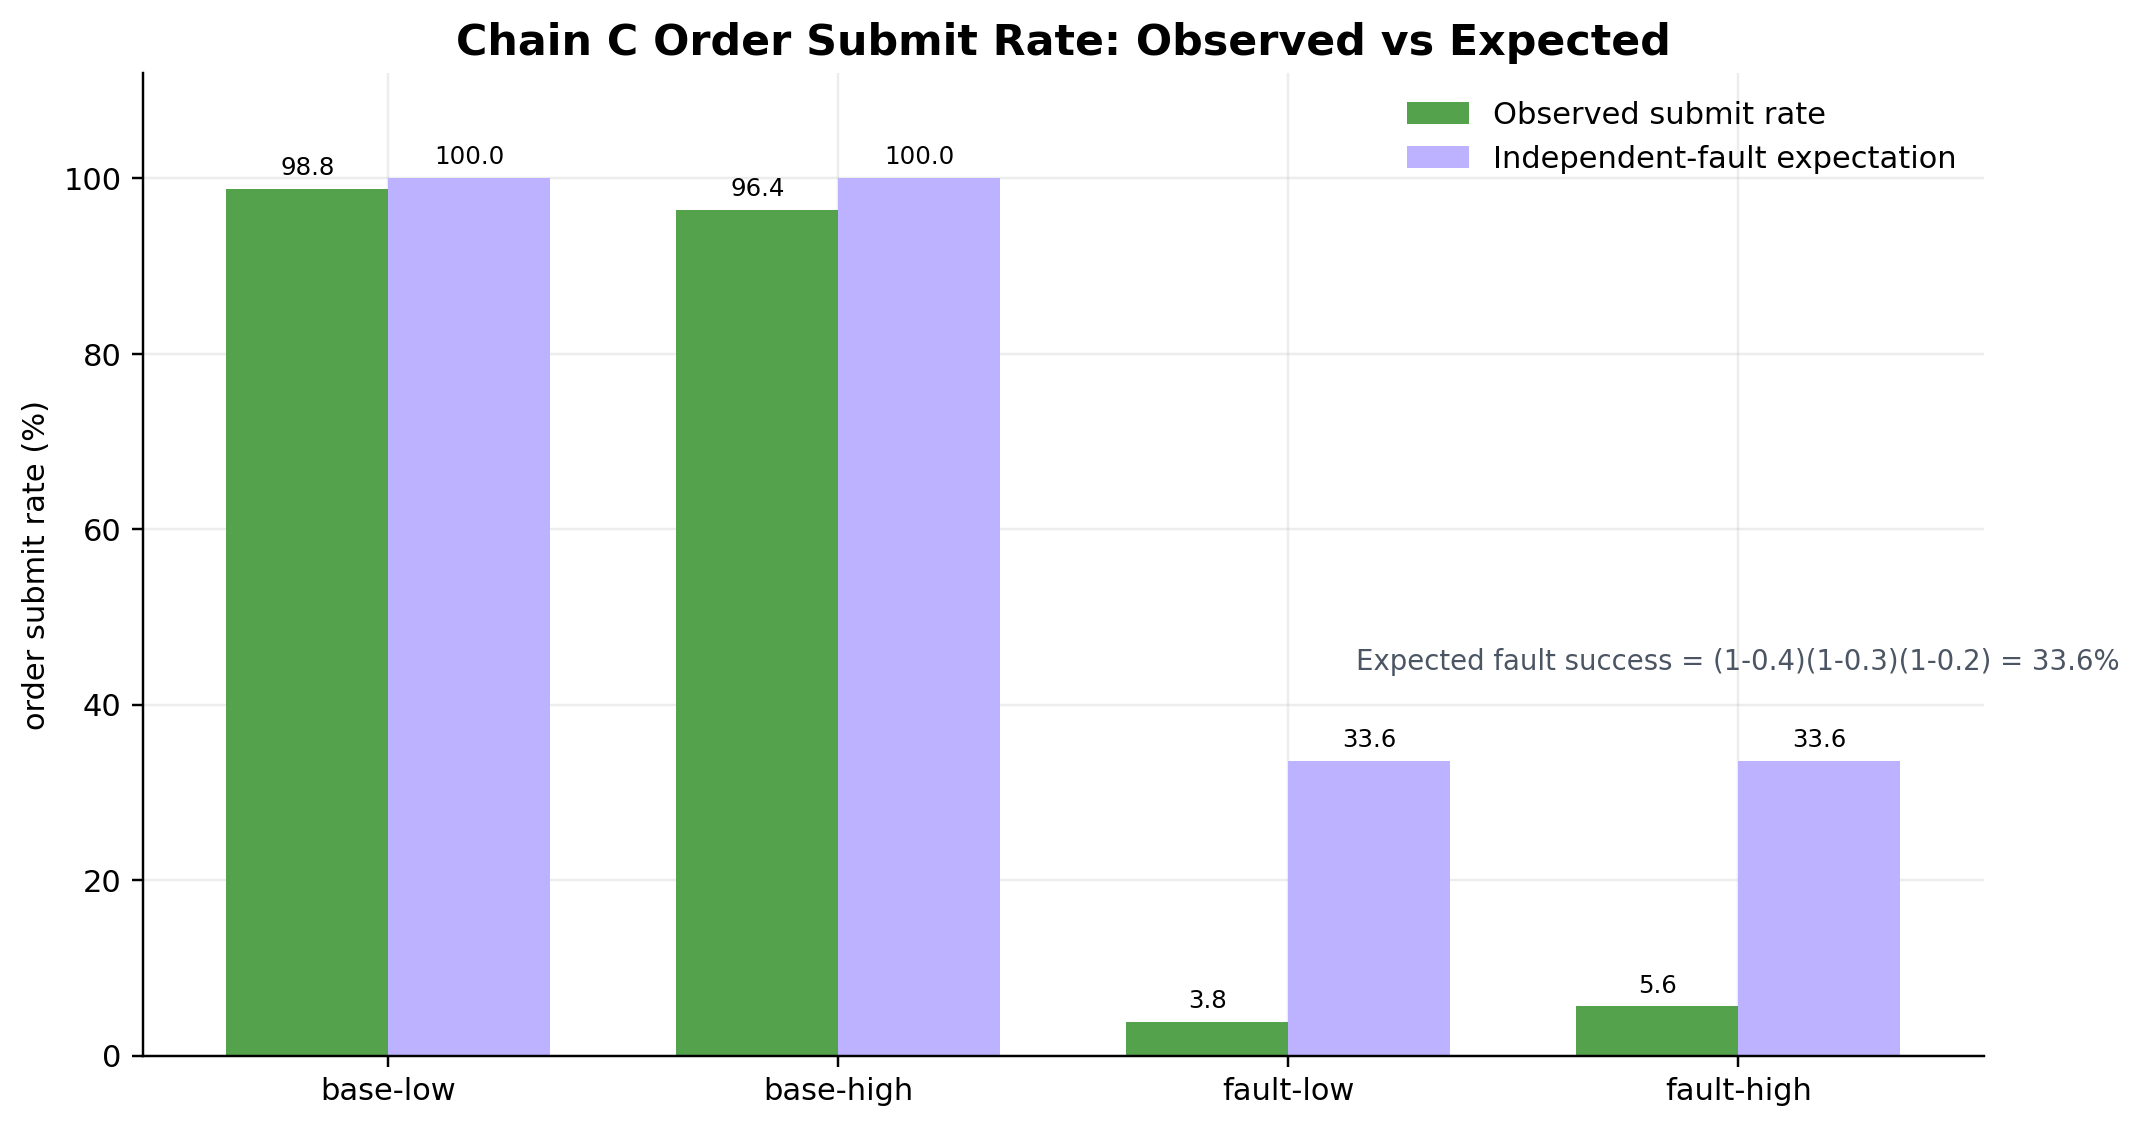
\includegraphics[width=\textwidth]{figures/case-chainc-submit-rate.png}
  \caption{链路 C 订单提交率实测值与理论预期对比}
  \label{fig:chainc-submit-rate}
\end{figure}

\section{实验有效性讨论}

为了保证实验结论可信，本文需要注意以下威胁。第一，LLM 输出具有不确定性，相同输入可能得到不同输出，因此业务质量指标应优先关注结构性变化，并保留请求样本。第二，外部 API 或模型网关可能波动，需要通过 baseline 和恢复窗口排除背景噪声。第三，本地机器资源不足可能造成高压组失败，必须结合系统指标解释。第四，低概率故障需要足够请求数，否则实际命中数不足以支撑结论。第五，如果后续启用 Trace 采样，需要保证故障 Trace 不被丢弃，或采用 tail-based sampling。

这些限制不会否定故障注入机制本身，但会影响实验结果的解释。本文实验已覆盖三条链路的四象限对比，并通过业务质量指标揭示了 HTTP 层不可见的退化；后续仍需补强资源监控、Trace 采样策略和图表化看板，以提升结果复查效率。
